\chapter{The summer record: July--September 2026}\label{ch:summer}

The October campaign measured in the rest of this part did not begin from
nothing. Between 19 July and 30 September the crypto-autoresearcher ledger
recorded 1{,}402 coordinator decisions on ECDLP and index calculus:
\begin{itemize}
\item July: 74 decisions on 20 experiments, 977 run directories;
\item August: 364 decisions on 92 experiments, 321 run directories;
\item September: 964 decisions on 449 experiments, 776 run directories.
\end{itemize}
Each decision names a verdict, the hypotheses and experiments it rules on,
and the evidence it cites. The dated index
(\art{research/ecdlp_jul_sep_index_20261029/}: \texttt{INDEX.json},
\texttt{INDEX.tsv}, and the generator \texttt{build\_index.py}) lays these
out together with the run-data path of each experiment. A decision is
counted as ECDLP work if its goal is one of 19 ECDLP goals or, when it names
no goal, if a target or evidence identifier carries an ECDLP family token.
That scope rule is a choice and is stated in the generator. Seven decisions
filed under late-September names carry October dates and are left out
of the counts above. Twenty-three decision files did not parse and are not
indexed.

\begin{figure}[t]
\centering
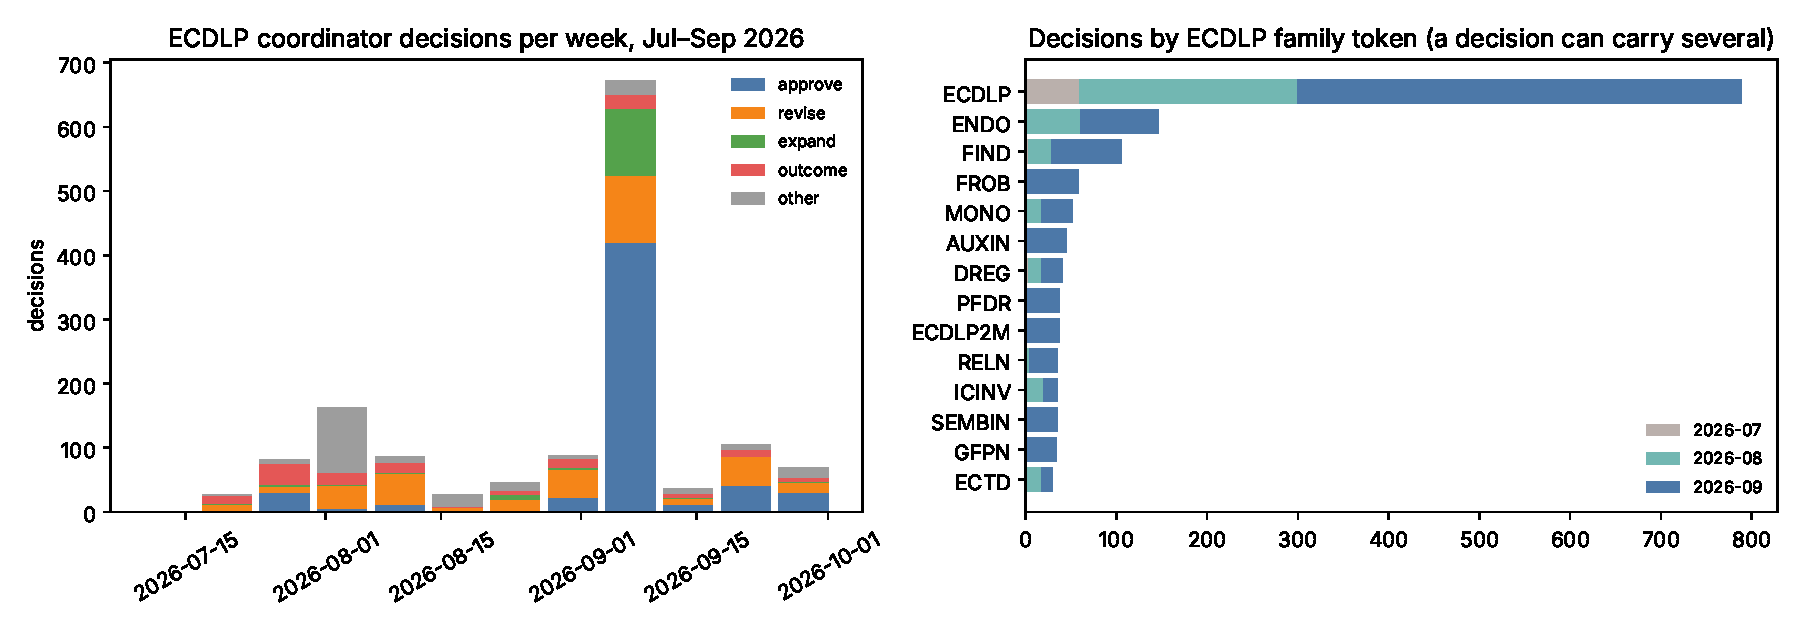
\includegraphics[width=\textwidth]{figures/fig-jul-sep.pdf}
\caption{ECDLP coordinator decisions, July--September 2026. Left: decisions
per week by verdict class. The class \emph{outcome} groups support,
reject\_scoped, weaken, inconclusive, supersede and pause. Right: decisions
per family token, by month; a decision can carry several tokens. The week
of 7 September holds 672 decisions, most of them approvals of frozen stage-0
contracts.}\label{fig:julsep}
\end{figure}

Most of this activity was process (Figure~\ref{fig:julsep}). Of the
1{,}402 decisions, 561 approve a contract, 267 revise one and 124 expand
one. About 157 carry an outcome on a hypothesis (support, reject, weaken,
inconclusive, supersede, pause or replicate). This chapter reports
those outcomes by theme, with decision identifiers so that each can be
traced. All results are at toy or derivation tier unless a scale is given.
None moved an exponent on a prime field.

\section{July: the first baseline and two retracted wins}

The ledger's first ECDLP decision, \texttt{DEC-20260719-001}, expanded a
toy Semaev $S_3$ Gröbner study (\texttt{EV-SEMAEV-001}). It had twelve runs
at 8--12 bits with a factor base of 14 points. The degree proxy stayed at
most 4 and the wall time stayed flat near 0.16\,s. The decision itself
noted that three bit sizes and two seeds cannot establish a trend.

Two supports followed on 26 July, and both were overturned the next day:
\begin{itemize}
\item \emph{Index calculus beats enumeration} (\texttt{H-IC-001}, 748 runs
  at 8--36 bits) was weakened by \texttt{DEC-20260727-008}. The criterion
  had been revised after the outcome. There were no decompositions at 20
  bits or above, so the measured descent time was the cost of a failed
  attempt. The relation cost was $2287\times$ the group order at 36 bits.
  The decision records: ``no asymptotic exponent moves''.
\item \emph{A structured factor base induces sparsity} (\texttt{H-STR-002})
  was weakened by \texttt{DEC-20260727-009}. Three headline instances had
  no run records. The one-variable ablation gave $\alpha=27,52,197,386$
  against $27,52,199,387$ for a random base, so the factor base induced
  nothing.
\end{itemize}
In the same week a generic-group classifier (\texttt{EXP-GGM-001}) had its
support revoked (\texttt{DEC-20260727-007}). It was a lookup table, and its
nine runs were byte-identical. Fixed-curve preprocessing showed no robust
gain over 72 runs (\texttt{DEC-20260726-001}, paused). A subresultant
degree exponent was measured at $\beta_{\rm deg}=0.5985$ against a gate of
$0.3$ (\texttt{DEC-20260728-003}, weakened).

Xedni-style lifting was closed in exact form (\texttt{DEC-20260724-021},
reject\_scoped): $P_{\rm lift}=(1-2/p+p^{-3})/(2p^3)$, so $\alpha=3$. This
is the result restated in Chapter~\ref{ch:obstructions}.

\section{August: yield, monodromy, oracles and transfers}

\paragraph{Yield matches the heuristic from below.} Semaev decomposition
yield at $m=2$ reached $0.80$, $0.98$ and $1.00$ of the $B^m/(m!N)$
heuristic at $p=1009$, $4001$ and $9001$ (\texttt{EV-YIELD-e1adbf}).
\texttt{DEC-20260804-9da614} weakened super-heuristic yield at $m=2$--$4$.
Structured bases gave small-$x$ $0.845$, arithmetic progression $0.658$
and random $0.563$, with no super-heuristic yield
(\texttt{DEC-20260804-2bfc30}). These measurements came before the
conservation proposition of Chapter~\ref{ch:cover}, which explains them: at
matched base size the mean is fixed. A complete $m=2$ index calculus solved
a discrete logarithm at $p=1009$ (\texttt{DEC-20260804-db75bb}). A
Fourier-flatness constant for the factor base was fitted as
$C(p)\sim p^{0.055}$--$p^{0.079}$ and recorded as an open problem
(\texttt{H-PSEUDO}). Eight proof routes were closed as non-proving.

\paragraph{BKK and meet in the middle: constant factors.} A BKK sparsity
argument promised a speedup of at least $(m+1)/2$
(\texttt{DEC-20260804-1825ea}). It measured $1.99988$ against $2.0$ at
$m=3$ on a smoke test. \texttt{DEC-20260806-26c0e8} then found the
multi-target window empty at the planned sizes and the gain about
$1.0$--$1.8\times$. Meet-in-the-middle structure gave $18\times$, which rho
dominates (\texttt{DEC-20260808-030b1f}). A degree-split claw lost its
advantage to a matched null, $R=0.0472$ against $0.0311$
(\texttt{DEC-20260801-005}). The decision reads: ``the instrument, not the
hypothesis, has been refuted''.

\paragraph{Monodromy.} The work that became Chapter~\ref{ch:cover} was
done in August:
\begin{itemize}
\item the $m=3$ derivation (\texttt{DEC-20260802-a51c82});
\item the all-$m$ theorem, supported as scoped and ``not closed''
  (\texttt{DEC-20260807-64df6a}, \texttt{KN-FIND-a8990a});
\item containment in $(\ZZ/2)^{m-2}$ at $m=4,5$ on eight curves, with zero
  exceptions in an exhaustive census of 2{,}915{,}514 triples at $p=103$
  (\texttt{DEC-20260830-0f8def});
\item monodromy $D_4$ for the $m=3$ symmetric-base cover
  (\texttt{DEC-20260830-1fb2e3}).
\end{itemize}
The fibre census was ruled blind to relation rate as an instrument
(\texttt{DEC-20260810-2f86db}, reject\_scoped), two months before the
census corollary proved why.

\paragraph{Oracles and transfers.} Two analysis-only results bounded the
oracle leads. Oracles C and D are simulable in the generic group model, and
A and B give no sub-birthday advantage (\texttt{DEC-20260804-3b4258},
support\_scoped). The doubling oracle was then shown equivalent to an
$x$-coordinate oracle (\texttt{DEC-20260806-08b9ed}). Three transfer and
invariant routes were closed:
\begin{itemize}
\item Isogeny transfer: the anomalous, MOV and Weil-descent families are
  invariants of the isogeny class (\texttt{DEC-20260804-2fae6a}).
\item Elkies augmentation: with $\ell\le23$ it matched a random-bijection
  null to within $0.004$ in all eight cells at 20--28 bits
  (\texttt{DEC-20260804-d0c452}).
\item CM: complex multiplication changes the lifted-height obstruction ``by
  exactly nothing'' (\texttt{DEC-20260810-2c7e3c}).
\end{itemize}
Within one isogeny class the over-dispersion of ECDLP-relevant statistics
traced to the 2-torsion type (\texttt{DEC-20260811-a3398a},
\texttt{KN-FIND-ddd982}).

\paragraph{Degree of regularity.} The boolean chained $m=3$ system was
run at $n=21$, $D=5$, and stopped at rank $265{,}950$ of a predicted
$268{,}674$ (\texttt{EV-DREG-4500cd}). The record calls this ``not evidence
about $d_{\rm reg}$ in either direction''. All six $n=15$ runs then
exceeded memory (\texttt{DEC-20260828-653923}). The certified
fall-degree results of Chapter~\ref{ch:falldegree} later replaced this
line.

Late August was spent on governance: budget ceilings, pauses and
zero-run successors. \texttt{DEC-20260820-0c8ffb} paused at the budget
ceiling. The ``fund every goal'' decisions of 28 August lifted the limits.

\section{September: tables, lifts, audits and the first binary costing}

\paragraph{Distinguished-point tables re-selected from the batch.} The
claim that a table of $T/2$ entries re-selected from solved walks matches a
static Bernstein--Lange table of $T$ was contradicted at $a=1/4$. It
reached $0.65$--$0.69\,T$ at steady state, with intervals excluding 1,
while paying $2.6$--$8.9\,T$ of working storage (\texttt{DEC-20260906-1f5b71},
weaken: ``a tradeoff point, not an improvement''). At $N=2^{24}$ the
feasibility crossing was then bracketed between $a=1/8$ and $a=3/16$
(\texttt{DEC-20260907-9b1b02}, \texttt{DEC-20260907-6d9427}). The result is
a ceiling only, with no online arm (\texttt{DEC-20260910-34e654}).

\paragraph{The canonical lift carries no logarithm.} The $p$-adic lift
statistic $D_1$ took exactly the values $\{0,8\}$ on 1{,}035 pairs at
$p=1009$, and the same in a third independent implementation and on a
second instance. It tracked precision $r=4,8,12$ exactly
(\texttt{DEC-20260903-256c7c}). The digit identity held in $1360/1360$
cases, and the Teichmüller contrast showed no inflation: all three ratio
intervals contain 1 (\texttt{DEC-20260911-74c9dc},
\texttt{DEC-20260912-2a626b}). Both results were recorded as ``no attack''.

\paragraph{Natural statistics are not biased enough.} An $L^1$ Fourier
registry over 406 cells and primes $4099$--$16{,}777{,}259$ falsified two
of its four predictions (\texttt{DEC-20260921-4516a0}, weaken):
\begin{itemize}
\item interval statistics: $\lambda=0.0806\pm0.0020$, against a
  prediction of at most $0.05$;
\item cosets and quadratic residues: $0.50$, against a prediction near 0.
\end{itemize}

\paragraph{Semaev degree and the Semaev 2015 / Nagao audits.} The
successful-subset loophole in the Semaev degree law was closed:
$\beta_{\rm work}=0.797$ worst case over 36 cells and 1{,}152 queries
(\texttt{DEC-20260929-780751}, reject\_scoped, \texttt{EV-SDEG-4a1c3d}).
The audits of Semaev's 2015 paper and Nagao's programme
(Chapter~\ref{ch:falldegree}) recorded these verdicts:
\begin{itemize}
\item eq.~(11)'s $\lambda$ is right to 1\% at $t=2$, but $P=1-e^{-\lambda}$
  fails by 18--22\% in the low-degree window (\texttt{DEC-20260913-3b51c8});
\item the typed-image ratio is not $m!$ at any of seven cells
  (\texttt{DEC-20260913-2386b5});
\item trace-parity confinement explains the whole deficit at $t=2$
  (\texttt{DEC-20260913-92aa48});
\item Nagao's memory claim fails at $n=571$, and 81 of the 120 flagged
  cells were an artifact of an incoherent memory pairing
  (\texttt{DEC-20260914-537000});
\item a published measurement claim, P3, fails under the corrected XOR
  product: the Semaev median is 2 in all eight cells, with the null at
  least one above it (\texttt{DEC-20260929-e37785}, reject\_scoped).
\end{itemize}

\paragraph{Prime-field degree versus yield.} A closed form for the first
fall degree of a digit-map presentation,
$d_{\rm ff}=m2^{m-1}+\lfloor(s-2^{m-1})/2\rfloor+1$, survived 26{,}000
instances with zero deviations. Its companion fall-dimension clause was
refuted by a certificate at $p=13$ (\texttt{DEC-20260904-1e27a2}). The
generator degree is $m2^{m-1}$, not $2m$, and the ``cells below rho'' of a
cost table had zero rows at $D_0$, so they were rejected
(\texttt{DEC-20260904-d47cd2}).

\paragraph{Frobenius-stable factor bases.} The stable subspaces are
exactly the ideals of $\FF_q[T]/(T^n-1)$, and the orbit count is exact on
14 of 14 cells (\texttt{DEC-20260922-5796b8},
\texttt{EV-FROB-d336b0}). The orbit gain is $n$, a constant factor. At
$n=131$ there are only four stable subspaces, and the orbit trick
\emph{loses} $57.0$--$96.0$ bits for $m=2$--$5$; at $n=163$ it loses
$72.7$--$121.7$ bits. Whether WDSat is blind to basis choice was never
measured, because 19 stage-0 launches failed.

\paragraph{The first costing of descended systems against rho.} The ICPERF
lane priced the descended algebraic normal form against the whole rho
budget on standard binary curves (\texttt{DEC-20260922-925da8},
\texttt{EV-ICPERF-784b25}). Forming the system alone exceeds rho by
$+6.3$ bits at $n=233$ and by $+40.8$ bits at $n=131$ (ECC2K-130).
Below $n\approx300$ the obstacle is building the system, not solving it.
The excess turns negative at $n=409$ and $571$ for $m\ge4$, and $m=2$
loses at every degree. This is the first September result priced against
rho. It is a model with measured inputs, not a solve.

\paragraph{Lanes without a result.} Several September lanes produced
approvals and redesigns but no measured outcome:
\begin{itemize}
\item SAT on summation systems, trapdoor detection, invariant calibrators
  and endomorphism decomposition, mostly frozen stage-0 contracts
  approved on 13 September;
\item the auxiliary-input census, whose run was ruled invalid as evidence
  because its controls were inadmissible and its escalation was generic to
  256-bit primes (\texttt{DEC-20260923-ce06a6});
\item EcGFp5 symmetrisation, where no $m=5$ ideal degree was measured
  (\texttt{DEC-20260923-d86ff2}), although the audit found that the curve's
  self-reported 323 bits recomputes to 322;
\item characteristic-2 quasi-subfield work, which found zero violations of
  its bound in about $340{,}000$ candidates and produced the derivation
  $\beta>1/2$ for every completely splitting $L$ (\texttt{KN-FIND-617d78}).
\end{itemize}
The certified binary refutations of Chapter~\ref{ch:falldegree} begin here:
$W_4$ refutes 62/62 at $n=17$ and 400/400 at $n=19$
(\texttt{DEC-20260924-e61f3b}, \texttt{DEC-20260926-901ea1}).

\begin{table}[p]
\centering\small
\setlength{\tabcolsep}{4pt}
\begin{tabular}{@{}llllp{4.6cm}@{}}
\toprule
month & theme & decision & verdict & recorded result \\
\midrule
Jul & IC beats enumeration & \texttt{DEC-20260727-008} & weaken & relation cost $2287\times$ the group order at 36 bits \\
    & structured factor base & \texttt{DEC-20260727-009} & weaken & $\alpha=27,52,197,386$ vs.\ random $27,52,199,387$ \\
    & subresultant degree & \texttt{DEC-20260728-003} & weaken & $\beta_{\rm deg}=0.5985$ vs.\ gate $0.3$ \\
    & xedni lifting & \texttt{DEC-20260724-021} & reject\_scoped & $\alpha=3$ \\
\addlinespace
Aug & Semaev yield, $m=2$ & \texttt{DEC-20260804-9da614} & weaken & $0.80$, $0.98$, $1.00$ of heuristic at $p=1009,4001,9001$ \\
    & BKK speedup & \texttt{DEC-20260806-26c0e8} & supersede claim & $1.0$--$1.8\times$, not $(m+1)/2$ \\
    & degree-split claw & \texttt{DEC-20260801-005} & weaken & $R=0.0472$ (null) vs.\ $0.0311$ \\
    & monodromy, $m=4,5$ & \texttt{DEC-20260830-0f8def} & support & 0 exceptions in 2{,}915{,}514 triples at $p=103$ \\
    & Elkies augmentation & \texttt{DEC-20260804-d0c452} & reject\_scoped & within $0.004$ of null, 8 cells, 20--28 bits \\
    & boolean $d_{\rm reg}$, $n=21$ & \texttt{DEC-20260815-6b806c} & supersede & rank $265{,}950$ of $268{,}674$; not evidence \\
\addlinespace
Sep & re-selected DP table & \texttt{DEC-20260906-1f5b71} & weaken & $0.65$--$0.69\,T$ at $a=1/4$ \\
    & canonical lift $D_1$ & \texttt{DEC-20260903-256c7c} & support & values exactly $\{0,8\}$ on 1{,}035 pairs; no attack \\
    & natural-statistic bias & \texttt{DEC-20260921-4516a0} & weaken & $\lambda=0.0806\pm0.0020$ vs.\ $\le0.05$ \\
    & Semaev degree loophole & \texttt{DEC-20260929-780751} & reject\_scoped & $\beta_{\rm work}=0.797$, 36 cells \\
    & Frobenius-stable bases & \texttt{DEC-20260922-5796b8} & support & loss of $57.0$--$96.0$ bits at $n=131$ \\
    & ICPERF costing & \texttt{DEC-20260922-925da8} & support & $+6.3$ ($n=233$) to $+40.8$ ($n=131$) bits over rho \\
\bottomrule
\end{tabular}
\caption[]{The summer record at a glance: one outcome decision per theme,
July--September 2026, with the number it recorded. Every row is
discussed above. Verdicts are the ledger's, shortened: ``weaken'' includes
\texttt{weaken\_h\_yield}, and ``supersede claim'' replaced the earlier
BKK support. Index: \art{research/ecdlp_jul_sep_index_20261029/INDEX.json}.}
\label{tab:summer}
\end{table}

\section{What the summer established}

Table~\ref{tab:summer} collects one outcome per theme. Four patterns run
through the 1{,}402 decisions:
\begin{enumerate}
\item \emph{No measured improvement over rho survived review.} Every
  July and August support that claimed a gain was weakened or revoked
  within days. The surviving gains are constant factors at toy scale.
\item \emph{The theory of Chapter~\ref{ch:cover} was found by
  measurement first.} The yield ratios at or below 1, the census ruled
  blind, and the exhaustive monodromy checks all preceded the proofs that
  explain them.
\item \emph{Most closures were instrument repairs.} A large share of the
  weaken and reject decisions say that a control, a metric or a criterion
  was wrong, not the hypothesis. This is the origin of the matched-null and
  replay rules of Chapter~\ref{sec:method}.
\item \emph{The binary line reached a priced verdict only in late
  September.} The ICPERF costing and the $W_4$ certificates opened the
  fall-degree and Koblitz work that the October campaign measured.
\end{enumerate}
These four patterns are the author's reading. The decisions cited above
are the record.
